% Created by tikzDevice version 0.12.3.1 on 2021-06-13 15:08:41
% !TEX encoding = UTF-8 Unicode
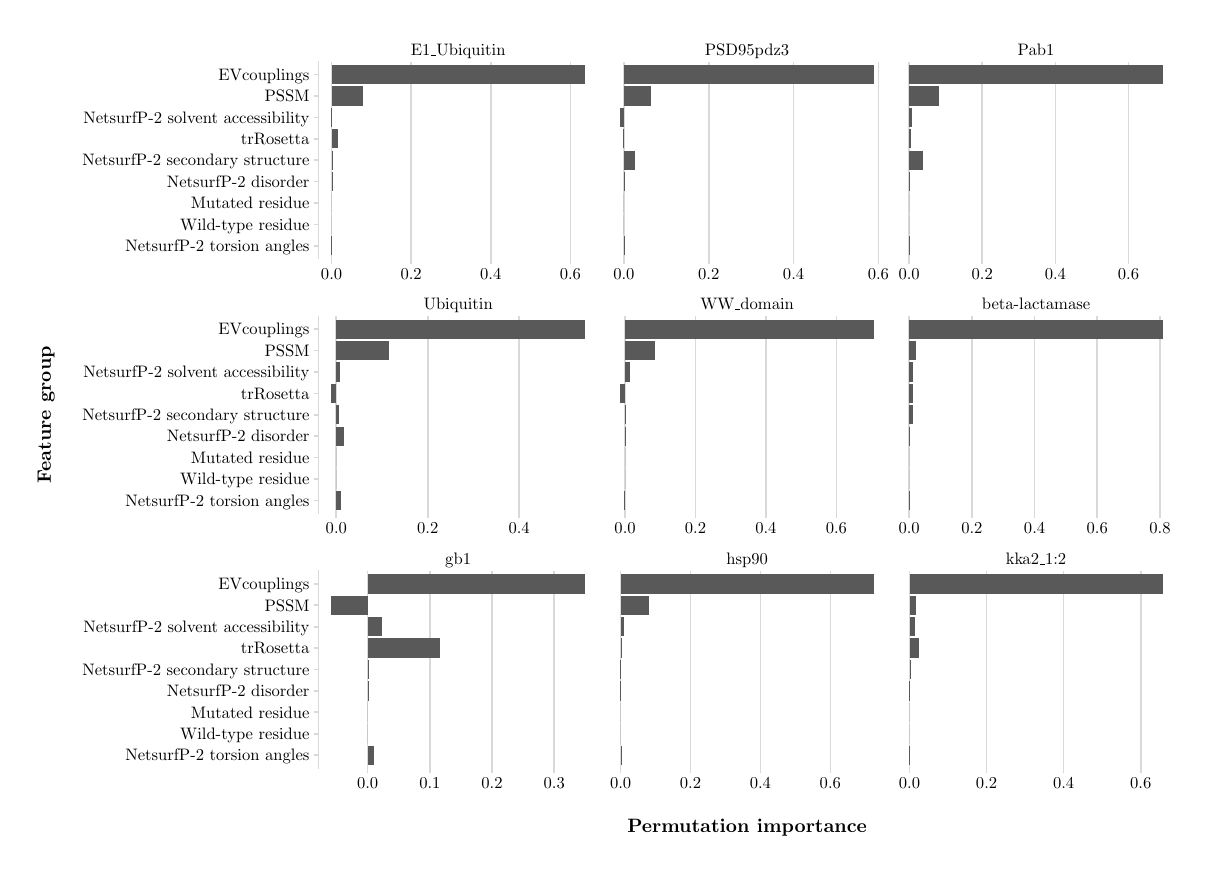
\begin{tikzpicture}[x=1pt,y=1pt]
\definecolor{fillColor}{RGB}{255,255,255}
\path[use as bounding box,fill=fillColor,fill opacity=0.00] (0,0) rectangle (418.34,295.82);
\begin{scope}
\path[clip] (105.09,212.35) rectangle (206.00,283.52);
\definecolor{drawColor}{gray}{0.85}

\path[draw=drawColor,line width= 0.6pt,line join=round] (109.81,212.35) --
	(109.81,283.52);

\path[draw=drawColor,line width= 0.6pt,line join=round] (138.58,212.35) --
	(138.58,283.52);

\path[draw=drawColor,line width= 0.6pt,line join=round] (167.35,212.35) --
	(167.35,283.52);

\path[draw=drawColor,line width= 0.6pt,line join=round] (196.12,212.35) --
	(196.12,283.52);
\definecolor{fillColor}{gray}{0.35}

\path[fill=fillColor] (109.81,252.19) rectangle (112.08,259.15);

\path[fill=fillColor] (109.81,267.66) rectangle (121.31,274.63);

\path[fill=fillColor] (109.69,259.93) rectangle (109.81,266.89);

\path[fill=fillColor] (109.81,244.46) rectangle (110.29,251.42);

\path[fill=fillColor] (109.81,236.72) rectangle (109.86,243.68);

\path[fill=fillColor] (109.68,213.51) rectangle (109.81,220.47);

\path[fill=fillColor] (109.81,275.40) rectangle (201.42,282.36);

\path[fill=fillColor] (109.81,221.25) rectangle (109.81,228.21);

\path[fill=fillColor] (109.81,228.98) rectangle (109.81,235.95);
\end{scope}
\begin{scope}
\path[clip] (105.09,120.33) rectangle (206.00,191.50);
\definecolor{drawColor}{gray}{0.85}

\path[draw=drawColor,line width= 0.6pt,line join=round] (111.53,120.33) --
	(111.53,191.50);

\path[draw=drawColor,line width= 0.6pt,line join=round] (144.56,120.33) --
	(144.56,191.50);

\path[draw=drawColor,line width= 0.6pt,line join=round] (177.59,120.33) --
	(177.59,191.50);
\definecolor{fillColor}{gray}{0.35}

\path[fill=fillColor] (109.68,160.17) rectangle (111.53,167.13);

\path[fill=fillColor] (111.53,175.64) rectangle (130.66,182.60);

\path[fill=fillColor] (111.53,167.90) rectangle (112.78,174.87);

\path[fill=fillColor] (111.53,152.43) rectangle (112.38,159.39);

\path[fill=fillColor] (111.53,144.70) rectangle (114.18,151.66);

\path[fill=fillColor] (111.53,121.49) rectangle (113.31,128.45);

\path[fill=fillColor] (111.53,183.38) rectangle (201.42,190.34);

\path[fill=fillColor] (111.53,129.22) rectangle (111.53,136.19);

\path[fill=fillColor] (111.53,136.96) rectangle (111.53,143.92);
\end{scope}
\begin{scope}
\path[clip] (105.09, 28.30) rectangle (206.00, 99.48);
\definecolor{drawColor}{gray}{0.85}

\path[draw=drawColor,line width= 0.6pt,line join=round] (122.85, 28.30) --
	(122.85, 99.48);

\path[draw=drawColor,line width= 0.6pt,line join=round] (145.33, 28.30) --
	(145.33, 99.48);

\path[draw=drawColor,line width= 0.6pt,line join=round] (167.80, 28.30) --
	(167.80, 99.48);

\path[draw=drawColor,line width= 0.6pt,line join=round] (190.27, 28.30) --
	(190.27, 99.48);
\definecolor{fillColor}{gray}{0.35}

\path[fill=fillColor] (122.85, 68.15) rectangle (149.00, 75.11);

\path[fill=fillColor] (109.68, 83.62) rectangle (122.85, 90.58);

\path[fill=fillColor] (122.85, 75.88) rectangle (128.20, 82.84);

\path[fill=fillColor] (122.85, 60.41) rectangle (123.05, 67.37);

\path[fill=fillColor] (122.85, 52.67) rectangle (122.92, 59.64);

\path[fill=fillColor] (122.85, 29.46) rectangle (125.12, 36.43);

\path[fill=fillColor] (122.85, 91.35) rectangle (201.42, 98.32);

\path[fill=fillColor] (122.85, 37.20) rectangle (122.85, 44.16);

\path[fill=fillColor] (122.85, 44.94) rectangle (122.85, 51.90);
\end{scope}
\begin{scope}
\path[clip] (209.50,212.35) rectangle (310.42,283.52);
\definecolor{drawColor}{gray}{0.85}

\path[draw=drawColor,line width= 0.6pt,line join=round] (215.46,212.35) --
	(215.46,283.52);

\path[draw=drawColor,line width= 0.6pt,line join=round] (246.11,212.35) --
	(246.11,283.52);

\path[draw=drawColor,line width= 0.6pt,line join=round] (276.76,212.35) --
	(276.76,283.52);

\path[draw=drawColor,line width= 0.6pt,line join=round] (307.40,212.35) --
	(307.40,283.52);
\definecolor{fillColor}{gray}{0.35}

\path[fill=fillColor] (215.27,252.19) rectangle (215.46,259.15);

\path[fill=fillColor] (215.46,267.66) rectangle (225.13,274.63);

\path[fill=fillColor] (214.09,259.93) rectangle (215.46,266.89);

\path[fill=fillColor] (215.46,244.46) rectangle (219.37,251.42);

\path[fill=fillColor] (215.46,236.72) rectangle (215.82,243.68);

\path[fill=fillColor] (215.46,213.51) rectangle (215.80,220.47);

\path[fill=fillColor] (215.46,275.40) rectangle (305.83,282.36);

\path[fill=fillColor] (215.46,221.25) rectangle (215.46,228.21);

\path[fill=fillColor] (215.46,228.98) rectangle (215.46,235.95);
\end{scope}
\begin{scope}
\path[clip] (209.50,120.33) rectangle (310.42,191.50);
\definecolor{drawColor}{gray}{0.85}

\path[draw=drawColor,line width= 0.6pt,line join=round] (215.87,120.33) --
	(215.87,191.50);

\path[draw=drawColor,line width= 0.6pt,line join=round] (241.32,120.33) --
	(241.32,191.50);

\path[draw=drawColor,line width= 0.6pt,line join=round] (266.77,120.33) --
	(266.77,191.50);

\path[draw=drawColor,line width= 0.6pt,line join=round] (292.22,120.33) --
	(292.22,191.50);
\definecolor{fillColor}{gray}{0.35}

\path[fill=fillColor] (214.09,160.17) rectangle (215.87,167.13);

\path[fill=fillColor] (215.87,175.64) rectangle (226.66,182.60);

\path[fill=fillColor] (215.87,167.90) rectangle (217.69,174.87);

\path[fill=fillColor] (215.72,152.43) rectangle (215.87,159.39);

\path[fill=fillColor] (215.87,144.70) rectangle (215.93,151.66);

\path[fill=fillColor] (215.31,121.49) rectangle (215.87,128.45);

\path[fill=fillColor] (215.87,183.38) rectangle (305.83,190.34);

\path[fill=fillColor] (215.87,129.22) rectangle (215.87,136.19);

\path[fill=fillColor] (215.87,136.96) rectangle (215.87,143.92);
\end{scope}
\begin{scope}
\path[clip] (209.50, 28.30) rectangle (310.42, 99.48);
\definecolor{drawColor}{gray}{0.85}

\path[draw=drawColor,line width= 0.6pt,line join=round] (214.27, 28.30) --
	(214.27, 99.48);

\path[draw=drawColor,line width= 0.6pt,line join=round] (239.53, 28.30) --
	(239.53, 99.48);

\path[draw=drawColor,line width= 0.6pt,line join=round] (264.78, 28.30) --
	(264.78, 99.48);

\path[draw=drawColor,line width= 0.6pt,line join=round] (290.04, 28.30) --
	(290.04, 99.48);
\definecolor{fillColor}{gray}{0.35}

\path[fill=fillColor] (214.27, 68.15) rectangle (214.90, 75.11);

\path[fill=fillColor] (214.27, 83.62) rectangle (224.43, 90.58);

\path[fill=fillColor] (214.27, 75.88) rectangle (215.57, 82.84);

\path[fill=fillColor] (214.09, 60.41) rectangle (214.27, 67.37);

\path[fill=fillColor] (214.19, 52.67) rectangle (214.27, 59.64);

\path[fill=fillColor] (214.25, 29.46) rectangle (214.27, 36.43);

\path[fill=fillColor] (214.27, 91.35) rectangle (305.83, 98.32);

\path[fill=fillColor] (214.27, 37.20) rectangle (214.27, 44.16);

\path[fill=fillColor] (214.27, 44.94) rectangle (214.27, 51.90);
\end{scope}
\begin{scope}
\path[clip] (313.92,212.35) rectangle (414.84,283.52);
\definecolor{drawColor}{gray}{0.85}

\path[draw=drawColor,line width= 0.6pt,line join=round] (318.51,212.35) --
	(318.51,283.52);

\path[draw=drawColor,line width= 0.6pt,line join=round] (344.94,212.35) --
	(344.94,283.52);

\path[draw=drawColor,line width= 0.6pt,line join=round] (371.37,212.35) --
	(371.37,283.52);

\path[draw=drawColor,line width= 0.6pt,line join=round] (397.80,212.35) --
	(397.80,283.52);
\definecolor{fillColor}{gray}{0.35}

\path[fill=fillColor] (318.51,252.19) rectangle (319.32,259.15);

\path[fill=fillColor] (318.51,267.66) rectangle (329.43,274.63);

\path[fill=fillColor] (318.51,259.93) rectangle (319.72,266.89);

\path[fill=fillColor] (318.51,244.46) rectangle (323.43,251.42);

\path[fill=fillColor] (318.51,236.72) rectangle (318.70,243.68);

\path[fill=fillColor] (318.51,213.51) rectangle (318.77,220.47);

\path[fill=fillColor] (318.51,275.40) rectangle (410.25,282.36);

\path[fill=fillColor] (318.51,221.25) rectangle (318.51,228.21);

\path[fill=fillColor] (318.51,228.98) rectangle (318.51,235.95);
\end{scope}
\begin{scope}
\path[clip] (313.92,120.33) rectangle (414.84,191.50);
\definecolor{drawColor}{gray}{0.85}

\path[draw=drawColor,line width= 0.6pt,line join=round] (318.53,120.33) --
	(318.53,191.50);

\path[draw=drawColor,line width= 0.6pt,line join=round] (341.19,120.33) --
	(341.19,191.50);

\path[draw=drawColor,line width= 0.6pt,line join=round] (363.84,120.33) --
	(363.84,191.50);

\path[draw=drawColor,line width= 0.6pt,line join=round] (386.50,120.33) --
	(386.50,191.50);

\path[draw=drawColor,line width= 0.6pt,line join=round] (409.16,120.33) --
	(409.16,191.50);
\definecolor{fillColor}{gray}{0.35}

\path[fill=fillColor] (318.53,160.17) rectangle (319.89,167.13);

\path[fill=fillColor] (318.53,175.64) rectangle (321.17,182.60);

\path[fill=fillColor] (318.53,167.90) rectangle (320.02,174.87);

\path[fill=fillColor] (318.53,152.43) rectangle (319.95,159.39);

\path[fill=fillColor] (318.53,144.70) rectangle (318.71,151.66);

\path[fill=fillColor] (318.51,121.49) rectangle (318.53,128.45);

\path[fill=fillColor] (318.53,183.38) rectangle (410.25,190.34);

\path[fill=fillColor] (318.53,129.22) rectangle (318.53,136.19);

\path[fill=fillColor] (318.53,136.96) rectangle (318.53,143.92);
\end{scope}
\begin{scope}
\path[clip] (313.92, 28.30) rectangle (414.84, 99.48);
\definecolor{drawColor}{gray}{0.85}

\path[draw=drawColor,line width= 0.6pt,line join=round] (318.65, 28.30) --
	(318.65, 99.48);

\path[draw=drawColor,line width= 0.6pt,line join=round] (346.50, 28.30) --
	(346.50, 99.48);

\path[draw=drawColor,line width= 0.6pt,line join=round] (374.35, 28.30) --
	(374.35, 99.48);

\path[draw=drawColor,line width= 0.6pt,line join=round] (402.19, 28.30) --
	(402.19, 99.48);
\definecolor{fillColor}{gray}{0.35}

\path[fill=fillColor] (318.65, 68.15) rectangle (321.92, 75.11);

\path[fill=fillColor] (318.65, 83.62) rectangle (320.82, 90.58);

\path[fill=fillColor] (318.65, 75.88) rectangle (320.61, 82.84);

\path[fill=fillColor] (318.65, 60.41) rectangle (318.94, 67.37);

\path[fill=fillColor] (318.62, 52.67) rectangle (318.65, 59.64);

\path[fill=fillColor] (318.51, 29.46) rectangle (318.65, 36.43);

\path[fill=fillColor] (318.65, 91.35) rectangle (410.25, 98.32);

\path[fill=fillColor] (318.65, 37.20) rectangle (318.65, 44.16);

\path[fill=fillColor] (318.65, 44.94) rectangle (318.65, 51.90);
\end{scope}
\begin{scope}
\path[clip] (105.09, 99.48) rectangle (206.00,108.28);
\definecolor{drawColor}{RGB}{0,0,0}

\node[text=drawColor,anchor=base,inner sep=0pt, outer sep=0pt, scale=  0.60] at (155.55,101.81) {gb1};
\end{scope}
\begin{scope}
\path[clip] (209.50, 99.48) rectangle (310.42,108.28);
\definecolor{drawColor}{RGB}{0,0,0}

\node[text=drawColor,anchor=base,inner sep=0pt, outer sep=0pt, scale=  0.60] at (259.96,101.81) {hsp90};
\end{scope}
\begin{scope}
\path[clip] (313.92, 99.48) rectangle (414.84,108.28);
\definecolor{drawColor}{RGB}{0,0,0}

\node[text=drawColor,anchor=base,inner sep=0pt, outer sep=0pt, scale=  0.60] at (364.38,101.81) {kka2\_1:2};
\end{scope}
\begin{scope}
\path[clip] (105.09,191.50) rectangle (206.00,200.30);
\definecolor{drawColor}{RGB}{0,0,0}

\node[text=drawColor,anchor=base,inner sep=0pt, outer sep=0pt, scale=  0.60] at (155.55,193.83) {Ubiquitin};
\end{scope}
\begin{scope}
\path[clip] (209.50,191.50) rectangle (310.42,200.30);
\definecolor{drawColor}{RGB}{0,0,0}

\node[text=drawColor,anchor=base,inner sep=0pt, outer sep=0pt, scale=  0.60] at (259.96,193.83) {WW\_domain};
\end{scope}
\begin{scope}
\path[clip] (313.92,191.50) rectangle (414.84,200.30);
\definecolor{drawColor}{RGB}{0,0,0}

\node[text=drawColor,anchor=base,inner sep=0pt, outer sep=0pt, scale=  0.60] at (364.38,193.83) {beta-lactamase};
\end{scope}
\begin{scope}
\path[clip] (105.09,283.52) rectangle (206.00,292.32);
\definecolor{drawColor}{RGB}{0,0,0}

\node[text=drawColor,anchor=base,inner sep=0pt, outer sep=0pt, scale=  0.60] at (155.55,285.86) {E1\_Ubiquitin};
\end{scope}
\begin{scope}
\path[clip] (209.50,283.52) rectangle (310.42,292.32);
\definecolor{drawColor}{RGB}{0,0,0}

\node[text=drawColor,anchor=base,inner sep=0pt, outer sep=0pt, scale=  0.60] at (259.96,285.86) {PSD95pdz3};
\end{scope}
\begin{scope}
\path[clip] (313.92,283.52) rectangle (414.84,292.32);
\definecolor{drawColor}{RGB}{0,0,0}

\node[text=drawColor,anchor=base,inner sep=0pt, outer sep=0pt, scale=  0.60] at (364.38,285.86) {Pab1};
\end{scope}
\begin{scope}
\path[clip] (  0.00,  0.00) rectangle (418.34,295.82);
\definecolor{drawColor}{gray}{0.85}

\path[draw=drawColor,line width= 0.6pt,line join=round] (122.85, 26.55) --
	(122.85, 28.30);

\path[draw=drawColor,line width= 0.6pt,line join=round] (145.33, 26.55) --
	(145.33, 28.30);

\path[draw=drawColor,line width= 0.6pt,line join=round] (167.80, 26.55) --
	(167.80, 28.30);

\path[draw=drawColor,line width= 0.6pt,line join=round] (190.27, 26.55) --
	(190.27, 28.30);
\end{scope}
\begin{scope}
\path[clip] (  0.00,  0.00) rectangle (418.34,295.82);
\definecolor{drawColor}{RGB}{0,0,0}

\node[text=drawColor,anchor=base,inner sep=0pt, outer sep=0pt, scale=  0.60] at (122.85, 20.92) {0.0};

\node[text=drawColor,anchor=base,inner sep=0pt, outer sep=0pt, scale=  0.60] at (145.33, 20.92) {0.1};

\node[text=drawColor,anchor=base,inner sep=0pt, outer sep=0pt, scale=  0.60] at (167.80, 20.92) {0.2};

\node[text=drawColor,anchor=base,inner sep=0pt, outer sep=0pt, scale=  0.60] at (190.27, 20.92) {0.3};
\end{scope}
\begin{scope}
\path[clip] (  0.00,  0.00) rectangle (418.34,295.82);
\definecolor{drawColor}{gray}{0.85}

\path[draw=drawColor,line width= 0.6pt,line join=round] (214.27, 26.55) --
	(214.27, 28.30);

\path[draw=drawColor,line width= 0.6pt,line join=round] (239.53, 26.55) --
	(239.53, 28.30);

\path[draw=drawColor,line width= 0.6pt,line join=round] (264.78, 26.55) --
	(264.78, 28.30);

\path[draw=drawColor,line width= 0.6pt,line join=round] (290.04, 26.55) --
	(290.04, 28.30);
\end{scope}
\begin{scope}
\path[clip] (  0.00,  0.00) rectangle (418.34,295.82);
\definecolor{drawColor}{RGB}{0,0,0}

\node[text=drawColor,anchor=base,inner sep=0pt, outer sep=0pt, scale=  0.60] at (214.27, 20.92) {0.0};

\node[text=drawColor,anchor=base,inner sep=0pt, outer sep=0pt, scale=  0.60] at (239.53, 20.92) {0.2};

\node[text=drawColor,anchor=base,inner sep=0pt, outer sep=0pt, scale=  0.60] at (264.78, 20.92) {0.4};

\node[text=drawColor,anchor=base,inner sep=0pt, outer sep=0pt, scale=  0.60] at (290.04, 20.92) {0.6};
\end{scope}
\begin{scope}
\path[clip] (  0.00,  0.00) rectangle (418.34,295.82);
\definecolor{drawColor}{gray}{0.85}

\path[draw=drawColor,line width= 0.6pt,line join=round] (318.65, 26.55) --
	(318.65, 28.30);

\path[draw=drawColor,line width= 0.6pt,line join=round] (346.50, 26.55) --
	(346.50, 28.30);

\path[draw=drawColor,line width= 0.6pt,line join=round] (374.35, 26.55) --
	(374.35, 28.30);

\path[draw=drawColor,line width= 0.6pt,line join=round] (402.19, 26.55) --
	(402.19, 28.30);
\end{scope}
\begin{scope}
\path[clip] (  0.00,  0.00) rectangle (418.34,295.82);
\definecolor{drawColor}{RGB}{0,0,0}

\node[text=drawColor,anchor=base,inner sep=0pt, outer sep=0pt, scale=  0.60] at (318.65, 20.92) {0.0};

\node[text=drawColor,anchor=base,inner sep=0pt, outer sep=0pt, scale=  0.60] at (346.50, 20.92) {0.2};

\node[text=drawColor,anchor=base,inner sep=0pt, outer sep=0pt, scale=  0.60] at (374.35, 20.92) {0.4};

\node[text=drawColor,anchor=base,inner sep=0pt, outer sep=0pt, scale=  0.60] at (402.19, 20.92) {0.6};
\end{scope}
\begin{scope}
\path[clip] (  0.00,  0.00) rectangle (418.34,295.82);
\definecolor{drawColor}{gray}{0.85}

\path[draw=drawColor,line width= 0.6pt,line join=round] (111.53,118.58) --
	(111.53,120.33);

\path[draw=drawColor,line width= 0.6pt,line join=round] (144.56,118.58) --
	(144.56,120.33);

\path[draw=drawColor,line width= 0.6pt,line join=round] (177.59,118.58) --
	(177.59,120.33);
\end{scope}
\begin{scope}
\path[clip] (  0.00,  0.00) rectangle (418.34,295.82);
\definecolor{drawColor}{RGB}{0,0,0}

\node[text=drawColor,anchor=base,inner sep=0pt, outer sep=0pt, scale=  0.60] at (111.53,112.94) {0.0};

\node[text=drawColor,anchor=base,inner sep=0pt, outer sep=0pt, scale=  0.60] at (144.56,112.94) {0.2};

\node[text=drawColor,anchor=base,inner sep=0pt, outer sep=0pt, scale=  0.60] at (177.59,112.94) {0.4};
\end{scope}
\begin{scope}
\path[clip] (  0.00,  0.00) rectangle (418.34,295.82);
\definecolor{drawColor}{gray}{0.85}

\path[draw=drawColor,line width= 0.6pt,line join=round] (215.87,118.58) --
	(215.87,120.33);

\path[draw=drawColor,line width= 0.6pt,line join=round] (241.32,118.58) --
	(241.32,120.33);

\path[draw=drawColor,line width= 0.6pt,line join=round] (266.77,118.58) --
	(266.77,120.33);

\path[draw=drawColor,line width= 0.6pt,line join=round] (292.22,118.58) --
	(292.22,120.33);
\end{scope}
\begin{scope}
\path[clip] (  0.00,  0.00) rectangle (418.34,295.82);
\definecolor{drawColor}{RGB}{0,0,0}

\node[text=drawColor,anchor=base,inner sep=0pt, outer sep=0pt, scale=  0.60] at (215.87,112.94) {0.0};

\node[text=drawColor,anchor=base,inner sep=0pt, outer sep=0pt, scale=  0.60] at (241.32,112.94) {0.2};

\node[text=drawColor,anchor=base,inner sep=0pt, outer sep=0pt, scale=  0.60] at (266.77,112.94) {0.4};

\node[text=drawColor,anchor=base,inner sep=0pt, outer sep=0pt, scale=  0.60] at (292.22,112.94) {0.6};
\end{scope}
\begin{scope}
\path[clip] (  0.00,  0.00) rectangle (418.34,295.82);
\definecolor{drawColor}{gray}{0.85}

\path[draw=drawColor,line width= 0.6pt,line join=round] (318.53,118.58) --
	(318.53,120.33);

\path[draw=drawColor,line width= 0.6pt,line join=round] (341.19,118.58) --
	(341.19,120.33);

\path[draw=drawColor,line width= 0.6pt,line join=round] (363.84,118.58) --
	(363.84,120.33);

\path[draw=drawColor,line width= 0.6pt,line join=round] (386.50,118.58) --
	(386.50,120.33);

\path[draw=drawColor,line width= 0.6pt,line join=round] (409.16,118.58) --
	(409.16,120.33);
\end{scope}
\begin{scope}
\path[clip] (  0.00,  0.00) rectangle (418.34,295.82);
\definecolor{drawColor}{RGB}{0,0,0}

\node[text=drawColor,anchor=base,inner sep=0pt, outer sep=0pt, scale=  0.60] at (318.53,112.94) {0.0};

\node[text=drawColor,anchor=base,inner sep=0pt, outer sep=0pt, scale=  0.60] at (341.19,112.94) {0.2};

\node[text=drawColor,anchor=base,inner sep=0pt, outer sep=0pt, scale=  0.60] at (363.84,112.94) {0.4};

\node[text=drawColor,anchor=base,inner sep=0pt, outer sep=0pt, scale=  0.60] at (386.50,112.94) {0.6};

\node[text=drawColor,anchor=base,inner sep=0pt, outer sep=0pt, scale=  0.60] at (409.16,112.94) {0.8};
\end{scope}
\begin{scope}
\path[clip] (  0.00,  0.00) rectangle (418.34,295.82);
\definecolor{drawColor}{gray}{0.85}

\path[draw=drawColor,line width= 0.6pt,line join=round] (109.81,210.60) --
	(109.81,212.35);

\path[draw=drawColor,line width= 0.6pt,line join=round] (138.58,210.60) --
	(138.58,212.35);

\path[draw=drawColor,line width= 0.6pt,line join=round] (167.35,210.60) --
	(167.35,212.35);

\path[draw=drawColor,line width= 0.6pt,line join=round] (196.12,210.60) --
	(196.12,212.35);
\end{scope}
\begin{scope}
\path[clip] (  0.00,  0.00) rectangle (418.34,295.82);
\definecolor{drawColor}{RGB}{0,0,0}

\node[text=drawColor,anchor=base,inner sep=0pt, outer sep=0pt, scale=  0.60] at (109.81,204.97) {0.0};

\node[text=drawColor,anchor=base,inner sep=0pt, outer sep=0pt, scale=  0.60] at (138.58,204.97) {0.2};

\node[text=drawColor,anchor=base,inner sep=0pt, outer sep=0pt, scale=  0.60] at (167.35,204.97) {0.4};

\node[text=drawColor,anchor=base,inner sep=0pt, outer sep=0pt, scale=  0.60] at (196.12,204.97) {0.6};
\end{scope}
\begin{scope}
\path[clip] (  0.00,  0.00) rectangle (418.34,295.82);
\definecolor{drawColor}{gray}{0.85}

\path[draw=drawColor,line width= 0.6pt,line join=round] (215.46,210.60) --
	(215.46,212.35);

\path[draw=drawColor,line width= 0.6pt,line join=round] (246.11,210.60) --
	(246.11,212.35);

\path[draw=drawColor,line width= 0.6pt,line join=round] (276.76,210.60) --
	(276.76,212.35);

\path[draw=drawColor,line width= 0.6pt,line join=round] (307.40,210.60) --
	(307.40,212.35);
\end{scope}
\begin{scope}
\path[clip] (  0.00,  0.00) rectangle (418.34,295.82);
\definecolor{drawColor}{RGB}{0,0,0}

\node[text=drawColor,anchor=base,inner sep=0pt, outer sep=0pt, scale=  0.60] at (215.46,204.97) {0.0};

\node[text=drawColor,anchor=base,inner sep=0pt, outer sep=0pt, scale=  0.60] at (246.11,204.97) {0.2};

\node[text=drawColor,anchor=base,inner sep=0pt, outer sep=0pt, scale=  0.60] at (276.76,204.97) {0.4};

\node[text=drawColor,anchor=base,inner sep=0pt, outer sep=0pt, scale=  0.60] at (307.40,204.97) {0.6};
\end{scope}
\begin{scope}
\path[clip] (  0.00,  0.00) rectangle (418.34,295.82);
\definecolor{drawColor}{gray}{0.85}

\path[draw=drawColor,line width= 0.6pt,line join=round] (318.51,210.60) --
	(318.51,212.35);

\path[draw=drawColor,line width= 0.6pt,line join=round] (344.94,210.60) --
	(344.94,212.35);

\path[draw=drawColor,line width= 0.6pt,line join=round] (371.37,210.60) --
	(371.37,212.35);

\path[draw=drawColor,line width= 0.6pt,line join=round] (397.80,210.60) --
	(397.80,212.35);
\end{scope}
\begin{scope}
\path[clip] (  0.00,  0.00) rectangle (418.34,295.82);
\definecolor{drawColor}{RGB}{0,0,0}

\node[text=drawColor,anchor=base,inner sep=0pt, outer sep=0pt, scale=  0.60] at (318.51,204.97) {0.0};

\node[text=drawColor,anchor=base,inner sep=0pt, outer sep=0pt, scale=  0.60] at (344.94,204.97) {0.2};

\node[text=drawColor,anchor=base,inner sep=0pt, outer sep=0pt, scale=  0.60] at (371.37,204.97) {0.4};

\node[text=drawColor,anchor=base,inner sep=0pt, outer sep=0pt, scale=  0.60] at (397.80,204.97) {0.6};
\end{scope}
\begin{scope}
\path[clip] (  0.00,  0.00) rectangle (418.34,295.82);
\definecolor{drawColor}{gray}{0.85}

\path[draw=drawColor,line width= 0.6pt,line join=round,line cap=rect] (105.09,212.35) --
	(105.09,283.52);
\end{scope}
\begin{scope}
\path[clip] (  0.00,  0.00) rectangle (418.34,295.82);
\definecolor{drawColor}{RGB}{0,0,0}

\node[text=drawColor,anchor=base east,inner sep=0pt, outer sep=0pt, scale=  0.60] at (101.84,214.92) {NetsurfP-2 torsion angles};

\node[text=drawColor,anchor=base east,inner sep=0pt, outer sep=0pt, scale=  0.60] at (101.84,222.66) {Wild-type residue};

\node[text=drawColor,anchor=base east,inner sep=0pt, outer sep=0pt, scale=  0.60] at (101.84,230.40) {Mutated residue};

\node[text=drawColor,anchor=base east,inner sep=0pt, outer sep=0pt, scale=  0.60] at (101.84,238.13) {NetsurfP-2 disorder};

\node[text=drawColor,anchor=base east,inner sep=0pt, outer sep=0pt, scale=  0.60] at (101.84,245.87) {NetsurfP-2 secondary structure};

\node[text=drawColor,anchor=base east,inner sep=0pt, outer sep=0pt, scale=  0.60] at (101.84,253.61) {trRosetta};

\node[text=drawColor,anchor=base east,inner sep=0pt, outer sep=0pt, scale=  0.60] at (101.84,261.34) {NetsurfP-2 solvent accessibility};

\node[text=drawColor,anchor=base east,inner sep=0pt, outer sep=0pt, scale=  0.60] at (101.84,269.08) {PSSM};

\node[text=drawColor,anchor=base east,inner sep=0pt, outer sep=0pt, scale=  0.60] at (101.84,276.81) {EVcouplings};
\end{scope}
\begin{scope}
\path[clip] (  0.00,  0.00) rectangle (418.34,295.82);
\definecolor{drawColor}{gray}{0.85}

\path[draw=drawColor,line width= 0.6pt,line join=round] (103.34,216.99) --
	(105.09,216.99);

\path[draw=drawColor,line width= 0.6pt,line join=round] (103.34,224.73) --
	(105.09,224.73);

\path[draw=drawColor,line width= 0.6pt,line join=round] (103.34,232.46) --
	(105.09,232.46);

\path[draw=drawColor,line width= 0.6pt,line join=round] (103.34,240.20) --
	(105.09,240.20);

\path[draw=drawColor,line width= 0.6pt,line join=round] (103.34,247.94) --
	(105.09,247.94);

\path[draw=drawColor,line width= 0.6pt,line join=round] (103.34,255.67) --
	(105.09,255.67);

\path[draw=drawColor,line width= 0.6pt,line join=round] (103.34,263.41) --
	(105.09,263.41);

\path[draw=drawColor,line width= 0.6pt,line join=round] (103.34,271.14) --
	(105.09,271.14);

\path[draw=drawColor,line width= 0.6pt,line join=round] (103.34,278.88) --
	(105.09,278.88);
\end{scope}
\begin{scope}
\path[clip] (  0.00,  0.00) rectangle (418.34,295.82);
\definecolor{drawColor}{gray}{0.85}

\path[draw=drawColor,line width= 0.6pt,line join=round,line cap=rect] (105.09,120.33) --
	(105.09,191.50);
\end{scope}
\begin{scope}
\path[clip] (  0.00,  0.00) rectangle (418.34,295.82);
\definecolor{drawColor}{RGB}{0,0,0}

\node[text=drawColor,anchor=base east,inner sep=0pt, outer sep=0pt, scale=  0.60] at (101.84,122.90) {NetsurfP-2 torsion angles};

\node[text=drawColor,anchor=base east,inner sep=0pt, outer sep=0pt, scale=  0.60] at (101.84,130.64) {Wild-type residue};

\node[text=drawColor,anchor=base east,inner sep=0pt, outer sep=0pt, scale=  0.60] at (101.84,138.37) {Mutated residue};

\node[text=drawColor,anchor=base east,inner sep=0pt, outer sep=0pt, scale=  0.60] at (101.84,146.11) {NetsurfP-2 disorder};

\node[text=drawColor,anchor=base east,inner sep=0pt, outer sep=0pt, scale=  0.60] at (101.84,153.85) {NetsurfP-2 secondary structure};

\node[text=drawColor,anchor=base east,inner sep=0pt, outer sep=0pt, scale=  0.60] at (101.84,161.58) {trRosetta};

\node[text=drawColor,anchor=base east,inner sep=0pt, outer sep=0pt, scale=  0.60] at (101.84,169.32) {NetsurfP-2 solvent accessibility};

\node[text=drawColor,anchor=base east,inner sep=0pt, outer sep=0pt, scale=  0.60] at (101.84,177.06) {PSSM};

\node[text=drawColor,anchor=base east,inner sep=0pt, outer sep=0pt, scale=  0.60] at (101.84,184.79) {EVcouplings};
\end{scope}
\begin{scope}
\path[clip] (  0.00,  0.00) rectangle (418.34,295.82);
\definecolor{drawColor}{gray}{0.85}

\path[draw=drawColor,line width= 0.6pt,line join=round] (103.34,124.97) --
	(105.09,124.97);

\path[draw=drawColor,line width= 0.6pt,line join=round] (103.34,132.71) --
	(105.09,132.71);

\path[draw=drawColor,line width= 0.6pt,line join=round] (103.34,140.44) --
	(105.09,140.44);

\path[draw=drawColor,line width= 0.6pt,line join=round] (103.34,148.18) --
	(105.09,148.18);

\path[draw=drawColor,line width= 0.6pt,line join=round] (103.34,155.91) --
	(105.09,155.91);

\path[draw=drawColor,line width= 0.6pt,line join=round] (103.34,163.65) --
	(105.09,163.65);

\path[draw=drawColor,line width= 0.6pt,line join=round] (103.34,171.39) --
	(105.09,171.39);

\path[draw=drawColor,line width= 0.6pt,line join=round] (103.34,179.12) --
	(105.09,179.12);

\path[draw=drawColor,line width= 0.6pt,line join=round] (103.34,186.86) --
	(105.09,186.86);
\end{scope}
\begin{scope}
\path[clip] (  0.00,  0.00) rectangle (418.34,295.82);
\definecolor{drawColor}{gray}{0.85}

\path[draw=drawColor,line width= 0.6pt,line join=round,line cap=rect] (105.09, 28.30) --
	(105.09, 99.48);
\end{scope}
\begin{scope}
\path[clip] (  0.00,  0.00) rectangle (418.34,295.82);
\definecolor{drawColor}{RGB}{0,0,0}

\node[text=drawColor,anchor=base east,inner sep=0pt, outer sep=0pt, scale=  0.60] at (101.84, 30.88) {NetsurfP-2 torsion angles};

\node[text=drawColor,anchor=base east,inner sep=0pt, outer sep=0pt, scale=  0.60] at (101.84, 38.62) {Wild-type residue};

\node[text=drawColor,anchor=base east,inner sep=0pt, outer sep=0pt, scale=  0.60] at (101.84, 46.35) {Mutated residue};

\node[text=drawColor,anchor=base east,inner sep=0pt, outer sep=0pt, scale=  0.60] at (101.84, 54.09) {NetsurfP-2 disorder};

\node[text=drawColor,anchor=base east,inner sep=0pt, outer sep=0pt, scale=  0.60] at (101.84, 61.82) {NetsurfP-2 secondary structure};

\node[text=drawColor,anchor=base east,inner sep=0pt, outer sep=0pt, scale=  0.60] at (101.84, 69.56) {trRosetta};

\node[text=drawColor,anchor=base east,inner sep=0pt, outer sep=0pt, scale=  0.60] at (101.84, 77.30) {NetsurfP-2 solvent accessibility};

\node[text=drawColor,anchor=base east,inner sep=0pt, outer sep=0pt, scale=  0.60] at (101.84, 85.03) {PSSM};

\node[text=drawColor,anchor=base east,inner sep=0pt, outer sep=0pt, scale=  0.60] at (101.84, 92.77) {EVcouplings};
\end{scope}
\begin{scope}
\path[clip] (  0.00,  0.00) rectangle (418.34,295.82);
\definecolor{drawColor}{gray}{0.85}

\path[draw=drawColor,line width= 0.6pt,line join=round] (103.34, 32.95) --
	(105.09, 32.95);

\path[draw=drawColor,line width= 0.6pt,line join=round] (103.34, 40.68) --
	(105.09, 40.68);

\path[draw=drawColor,line width= 0.6pt,line join=round] (103.34, 48.42) --
	(105.09, 48.42);

\path[draw=drawColor,line width= 0.6pt,line join=round] (103.34, 56.15) --
	(105.09, 56.15);

\path[draw=drawColor,line width= 0.6pt,line join=round] (103.34, 63.89) --
	(105.09, 63.89);

\path[draw=drawColor,line width= 0.6pt,line join=round] (103.34, 71.63) --
	(105.09, 71.63);

\path[draw=drawColor,line width= 0.6pt,line join=round] (103.34, 79.36) --
	(105.09, 79.36);

\path[draw=drawColor,line width= 0.6pt,line join=round] (103.34, 87.10) --
	(105.09, 87.10);

\path[draw=drawColor,line width= 0.6pt,line join=round] (103.34, 94.84) --
	(105.09, 94.84);
\end{scope}
\begin{scope}
\path[clip] (  0.00,  0.00) rectangle (418.34,295.82);
\definecolor{drawColor}{RGB}{0,0,0}

\node[text=drawColor,anchor=base,inner sep=0pt, outer sep=0pt, scale=  0.70] at (259.96,  4.86) {\bfseries Permutation importance};
\end{scope}
\begin{scope}
\path[clip] (  0.00,  0.00) rectangle (418.34,295.82);
\definecolor{drawColor}{RGB}{0,0,0}

\node[text=drawColor,rotate= 90.00,anchor=base,inner sep=0pt, outer sep=0pt, scale=  0.70] at (  8.39,155.91) {\bfseries Feature group};
\end{scope}
\end{tikzpicture}%
